% !Mode:: "TeX:UTF-8" 
\section{国内外在该方向的研究现状及分析}
\subsection{国内外研究现状}

“不确定性”和“风险”是各个学术领域均比较关注的一个研究问题。本节简要归纳不确定性的分类、度量和各类不同的处理对策,思路如图~\ref{uc_ways}~所示。

\begin{figure}[htbp]
\centering
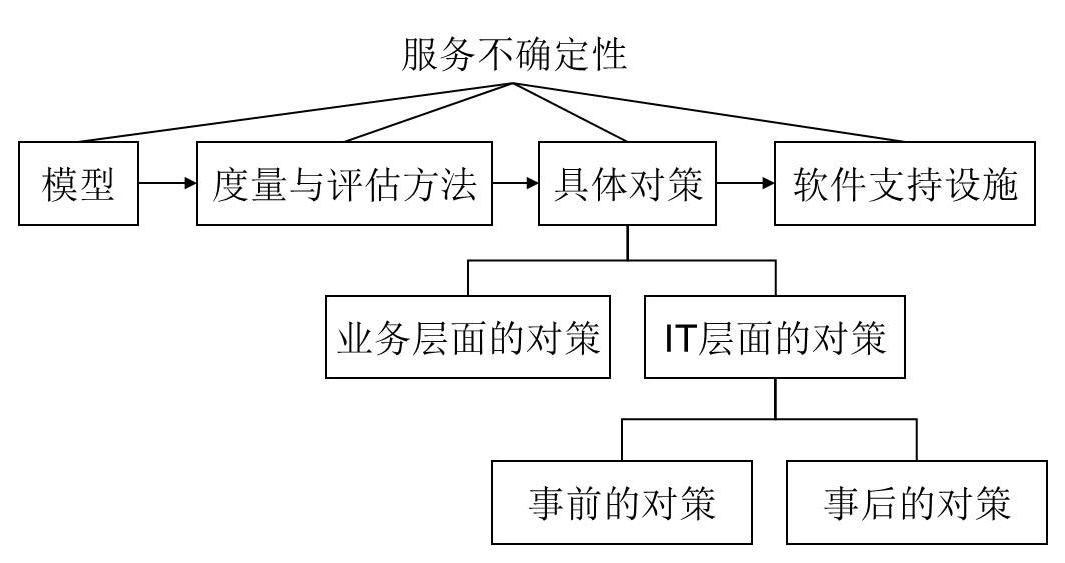
\includegraphics[width = 0.4\textwidth]{uc_ways}
\caption{国内外研究现状综述的线索}\label{uc_ways}
\vspace{-1em}
\end{figure}

按照这个思路,目前国外的研究现状主要分为以下4大部分。

(1)~服务不确定性的描述、度量与评估方法

在按需服务环境中,客户对服务的使用通常建立在动态订阅基础上,客户与服务提供者在服务执行之前需要保证他们之间在性能、可靠性和可用性等~QoS~方面的协议。为了及时发现客户提出的质量期望与服务实现支持的质量之间潜在的不一致,在不同的情境下需要由客户、服务提供者、或者由他们共同执行有关分析。由于经济和实践方面的原因,需要对服务的~QoS~参数进行度量和监测,及时检查约定的服务级别和在~SLA~管理过程中汇报给相关参与者。~Web Service Level Agreement (WSLA)~框架旨在定义和监测~web~服务的~SLA~,标准的WSLA框架基于~XML Schema~定义灵活和可扩展的描述语言和可以监控不同~SLA~的运行时体系架构\citeup{keller2003wsla}。

针对服务运行时可能发生的不确定性,研究者从不同角度提出了分类模式。文献\cite{kokash2007evaluating}将其分为服务/数据/用户缺失、非期望的服务行为、性能问题、协议违反等类型。文献\cite{chan2009fault}从物理~(physical)~、开发~(development)~、交互~(interaction)~三个方面将服务的故障分为13个小类别,并对其原因和影响进行了全面的分析。文献针对~web~应用层面、~web service~层面、基础设施和中间件层面对可能的服务执行故障分为9类,例如~QoS~违反、~WS~执行失败、~WS~协调错误、网络错误等\citeup{ardagna2006faults}。

相关研究还包括基于SLA的服务风险度量与估算方法\citeup{michalk2010risk}、面向~SLA~一致性分析的自动化算法\citeup{yang2003compatibility}等,以协助客户/提供者发现不确定性以及造成的影响。

(2)~业务层面的不确定性处理对策

业务层面的不确定性主要来自于客户需求、服务资源可用性、外界业务环境的变化,而且与领域密切相关,不同领域的不确定性具有较大差别。这里以传统的供应链服务为例进行简要分析。供应链中的不确定性主要包括需求的不确定性、供应的不确定性和制造上的不确定性,可能导致整个供应链成本的升高、利用率的降低以及企业绩效风险的增加。针对需求的不确定性,单一的参与者可以通过贸易伙伴间的信息共享\citeup{yu2001benefits}、需求预测辅助的库存优化方法来解决;也有一些学者提出事先在供应链各类参与者之间建立合理协议来促进他们之间的协调\citeup{chan2006early}。针对供给方面的不确定性,应对策略主要在于优化供应商的选择\citeup{amid2011weighted},与供应商维持良好的合作关系,以确保供应商能够长期配合,并以签订的方式,明确补偿措施,降低供给过程中的不确定因素。从生产制造的角度,也可以对订单处理、物料、组装生产、运输和装置的前置时间控制在合理范围\citeup{lambrechts2011time},降低动作系统的复杂度以减少人工出错的机会,定期维护相关设备降低故障风险。在以上研究基础上,一些学者进一步讨论了各种不确定性对于供应链的整合(包括顾客整合,供应商整合和内部整合)的影响\citeup{prajogo2011supply}。

(3)~IT~层面的不确定性处理对策:事前

在软件层面,可采用可靠性保障的方法来解决~web~服务中的不确定性问题\citeup{subramanian2008enhancement},在最初构建服务方案时就考虑可能面临的风险,将可靠性、不确定性等因素加入到服务选择与服务组合模型/算法中,以降低未来执行中的风险。可使用~Stochastic Petri Nets~等工具对~Web~服务组合方案进行建模,以计算组合服务的~reliability\citeup{zhong2008reliability}~,或者考虑服务发生风险时的依赖关系\citeup{liu2009risk},以此作为服务组合的可靠性优化依据,进而通过~Markov~决策过程~(MDP)~等方法来选择最符合客户风险偏好的可靠服务\citeup{harney2008selective}\citeup{gao2011reliability}。

在软件层面,软件服务的不确定性与其可靠性息息相关。软件可靠性领域通常利用基于概率统计的不确定理论对软件可靠性进行建模,通过对软件故障过程分析和相应处理\citeup{zhangyongqiang2006},因此,为了在服务执行产生不确定事件时能够通过恢复机制来保障可靠性\citeup{chan2009design},可基于冗余策略预先配置备用服务或多个替代配置方案(配置树、执行计划)来提升服务方案的容错能力\citeup{kokash2006service},目标是使服务方案具备自我治愈的能力\citeup{ardagna2006faults}。当现有服务无法正常执行时直接由备选服务接替执行,也可采用备选流程的方式,在当前流程出现问题时直接切换到备选流程。为此需在服务建模阶段考虑各种不确定性,对建模元素的实现机制和应用场景进行扩展以提高模型描述能力和适应性\citeup{fan2002service}。

除此之外,~Web~服务过程中的不确定性也可以用补偿流程的方式来处理\citeup{fensel2002web},即:当执行中出现可预料的不确定性时可以按预先指定的流程执行相应的补偿操作从而使服务达到预期的解决效果。这些研究的目标是使服务方案逐渐具备越来越高的自我治愈~(self-healing)~的能力\citeup{ardagna2006faults}。

(4)~IT~层面的不确定性处理对策:事后

虽然SOA提供了一种通过规范说明和发布、发现、选择及组装独立开发的软件组件来构造复杂分布式系统的方法,由于服务环境各方面因素的不确定性,导致在执行过程中可能出现计划服务不可用的情况。在这种情况下,目前研究分别采用服务替换、服务重组等服务重配置方法、恢复与补偿机制等策略来应用执行中可能出现的不确定性\citeup{erradi2006recovery}。

服务替换是指当某个服务不可用时,如何用其他服务替代以维持整个服务过程的完整性和有效性\citeup{li2011petri}\citeup{athanasopoulos2009service}。服务的替换主要考虑服务的功能和非功能特性(主要是质量特性)。功能方面主要基于服务的参数类型等静态属性和动态行为特性\citeup{bordeaux2005two}的匹配保证替换前后服务过程功能的一致性,而非功能方面主要基于客户在QoS偏好对服务效用进行度量来保证和优化替换后的服务质量\citeup{claro2005selecting}。此外还有基于context的手段\citeup{pathak2007context}对服务的可替换性进行判断。

服务重组是指服务过程的重新组合。根据重组方式的不同,可以分为服务的大规模重选取和服务路径的重规划。服务重选取通常是大规模进行的,而服务路径的重规划是指将服务的全部或者部分流程进行重新规划,根据执行过程中所发生的不确定性的种类和严重程度而形成新的执行路径,服务的重规划通常包含了对于服务的重选取。文献\cite{bouhini2010discovery}使用服务片段作为重规划的基本单元以提升效率。文献\cite{bucchiarone2010design}提出了一组系统化的原则和指南,指导设计者如何构造/重规划适应变化的服务。

根据服务重组范围的不同,可以分为服务的完全重组和部分重组两种。完全重组是指在服务执行过程中出现不确定性时,有必要时将撤销或者作废服务过程中的已执行部分,而对整个服务过程进行重规划或者重选取,其代价至少为全新服务组合的代价,因此常常采用部分重组,即针对不同具体情况对服务过程中的部分环节或者子过程进行重规划或者重选取,使得调整后的结果能够满足预期的约束目标。当具体不确定性发生时,服务提供者通常期望以最小代价的改动使得服务过程恢复到满足期望的状态。因此常用的方法是对服务过程中处于不同执行阶段的部分进行划分,并在每次尝试失败后逐渐扩大考虑的范围,每次尝试中都期望在尽量小的范围内弥补甚至消失不确定性产生的后果\citeup{zhai2009soa}。还可使用修补技术对当前服务组合方案进行改变和增强,使之适应各类故障\citeup{yan2010self}。另外,可根据服务执行反馈的状况,采用进行持续规划~(continual planning)\citeup{kaldeli2011continual}~,以适应执行过程中出现的各类不确定情况。

\subsection{国内外文献综述的简析}
如上所述,目前关于服务不确定性的研究已经有了丰富的研究,但尚显不足。

(1)~大部分研究者站在软件服务的开发、运行和维护的角度上,探讨“当某服务执行出现异常”之前或之后如何应对。而本课题站在客户或者中介方的角度,他们作为服务的使用者,不可能也无需了解软件服务的内部执行细节,只是从外部观测到各类异常的发生,而无法得知造成异常的原因(例如服务器内部出错、网络出错等)。在这种情况下,通过各类不确定性的决策方法,提高第三方服务中介所构造的整体服务方案适应不确定性的能力,是本课题的研究重点,也是区别于传统研究的观点之一。

此类问题归纳起来,目前研究主要分为两类:
a)~建模阶段对服务模型进行抗风险能力的增强,一旦运行时发现问题即可按预案进行应对;
b)~运行阶段对相关服务进行替换、重组或修补,并确保操作前后服务功能和QoS的一致性。
针对此类问题,尚有以下两点不足:
a)~关注替换、重组、修补等单一决策动作如何操作、如何实施,对哪种动作的效果最优的考虑显得不足;
b)~决策目标定位在服务功能的相容性和~QoS~的可保障性,较少从经济角度考虑不确定性带来的时间和成本方面的损失。

(2)~目前的研究通常将~business~和~IT~层面的不确定性割裂开来,分别研究。例如,针对供应链中的需求/供给/制造的不确定性,研究业务层面如何应对;针对底层的~web service~和服务系统执行中的出错、延迟、失败等不确定性,研究软件层面如何应对。但是二者本质上是有联系的,将它们关联起来并建立映射,是本课题的另一个观点。

针对此类问题,目前的研究主要是针对不同的业务情况采取不同的方法,其不足体现在两个方面:a)~没有对业务的不确定性进行系统化的分类处理,以至于不确定性的处理方案没有重用性和对处理结果统一的价值度量;b)~完全停留在~business~层面纯手工进行决策,忽略了~IT~手段可以辅助业务不确定性的决策,效率低下并且无法准确量化不确定性的决策的代价。

本课题尝试着从以上两点入手展开研究,解决服务不确定性决策的优化问题,并将服务层面的不确定性与业务层目标结合起来,寻求处理不确定性的最优决策动作。

%服务执行过程中的典型动态自适应策略包括:服务替换、服务重组等服务重配置方法、恢复与补偿机制等策略\citeup{erradi2006recovery}。服务替换考虑服务的功能和非功能特性,基于服务的参数类型等静态属性和动态行为特性的匹配保证替换前后服务过程功能的一致性,基于客户的QoS偏好对服务效用进行度量来保证和优化替换后的服务质量\citeup{athanasopoulos2009service},并引入context对服务的可替换性进行判断\citeup{pathak2007context}。

%服务重组分为服务的大规模重选取和服务路径的重规划。文献\cite{bouhini2010discovery}使用服务片段作为重规划的基本单元以提升效率,文献\cite{bucchiarone2010design}提出了一组系统化的原则和指南,指导设计者如何构造/重规划适应变化的服务。为降低重组代价,对服务过程内处于不同执行状态的部分进行划分,每次尝试都期望在尽量小范围内弥补不确定性产生的后果,并在尝试失败后逐渐扩大重组范围\citeup{zhai2009soa}。还可使用修补技术对当前服务组合方案进行改变和增强,使之适应各类故障\citeup{yan2010self}。还可根据服务执行反馈的状况,采用进行持续规划\citeup{kaldeli2011continual},以适应执行过程中出现的各类不确定情况。

%在按需服务环境中,服务执行之前供需双方在性能、可靠性和可用性等~QoS~方面达成服务级别协议~(SLA)~。目前得以广泛应用的~Web Service Level Agreement (WSLA)~是一种用于定义和监测~web~服务的~SLA~描述语言和框架\citeup{keller2003wsla},为~SLA~的建模、扩展、度量和监控提供支持。文献\cite{kokash2007evaluating}\cite{chan2009fault}\cite{ardagna2006faults}对服务运行时可能发生的不确定性进行了不同角度的分类,从不确定性发生的层次(应用层面、服务层面、基础设施/中间件层面)、不确定性发生时的表现(服务/数据缺失、非期望的服务行为、性能问题、协议违反)等方面阐述了不确定性的含义,通过基于SLA的风险度量与估算方法协助发现不确定性及其影响\citeup{michalk2010risk}。

%服务不确定性与其可靠性息息相关,因此可采用可靠性保障的方法来解决~web~服务中的不确定性问题\citeup{subramanian2008enhancement},在最初构建服务方案时就考虑可能面临的风险,将可靠性、不确定性等因素加入到服务选择与服务组合模型/算法中,以降低未来执行中的风险。使用随机~Petri~网等工具对~web~服务组合方案进行建模并计算其可靠性\citeup{zhong2008reliability},或者将服务发生风险时的依赖关系作为服务组合的可靠性优化依据\citeup{liu2009risk},通过~Markov~决策过程(MDP)等方法来选择最符合客户风险偏好的可靠服务\citeup{harney2008selective}\citeup{gao2011reliability}。

%为了在服务执行产生不确定事件时能够通过恢复机制来保障可靠性[18],可基于冗余策略预先配置备用服务或多个替代配置方案(配置树、执行计划)来提升服务方案的容错能力[19],当现有服务无法正常执行时直接由备选服务接替执行,从而减少服务重选取的复杂性。除单个备选服务外,也可以采用备选流程的方式,在当前流程出现问题时直接切换到备选流程,从而避免了服务重规划的复杂性。为了实现这一点,需要在建模阶段就充分考虑各种不确定性,通过传统活动网络的方式、协调机制、反馈机制等手段进行建模,甚至对建模元素的实现机制和应用场景进行扩展[20]以提高模型描述能力和适应性。
